%%%%%%%%%%%%%%%%%%%%%%%%%%%%%%%%%%%%%%%%%
% Professional Mathematical Presentation Template
% 
% This template uses the beamer class with the Madrid theme
% and a custom color scheme for a clean, professional look
% that works well with mathematical content.
%%%%%%%%%%%%%%%%%%%%%%%%%%%%%%%%%%%%%%%%%
\documentclass[aspectratio=169]{beamer} % 16:9 aspect ratio (modern)
% Theme settings
\usetheme{Madrid}
\usecolortheme{default}
%\usetikzlibrary{arrows.meta}
\usepackage[dvipsnames]{xcolor}
\usepackage{forest}
\definecolor{primcolor}{RGB}{25,50,100} % Dark blue
\setbeamercolor{structure}{fg=primcolor}
\setbeamercolor{frametitle}{bg=primcolor!15, fg=primcolor}
\setbeamercolor{title}{fg=white} % White title text for contrast
\setbeamercolor{subtitle}{fg=white} % White subtitle text
\setbeamercolor{author}{fg=primcolor} % White author text
\setbeamercolor{date}{fg=primcolor} % White date text
\setbeamercolor{institute}{fg=primcolor} % White institute text
% Font settings
\usefonttheme{professionalfonts}
\usefonttheme{serif}
% Package imports
\usepackage{amsmath, amsfonts, amssymb, amsthm} % Math packages
\usepackage{mathtools} % Enhanced math tools
\usepackage{bm} % Bold math symbols
\usepackage{graphicx} % For images
\usepackage{booktabs} % Professional tables
\usepackage{tikz} % For diagrams
\usetikzlibrary{arrows, positioning, matrix, decorations.pathreplacing}
% Use beamer's theorem styles
\setbeamertemplate{theorem}[ams style]
\setbeamertemplate{theorems}[numbered]
% Remove navigation symbols
\setbeamertemplate{navigation symbols}{}
% Custom footer
\setbeamertemplate{footline}{
  \leavevmode%
  \hbox{%
  \begin{beamercolorbox}[wd=.333333\paperwidth,ht=2.25ex,dp=1ex,center]{author in head/foot}%
    \usebeamerfont{author in head/foot}\insertshortauthor
  \end{beamercolorbox}%
  \begin{beamercolorbox}[wd=.333333\paperwidth,ht=2.25ex,dp=1ex,center]{title in head/foot}%
    \usebeamerfont{title in head/foot}\insertshorttitle
  \end{beamercolorbox}%
  \begin{beamercolorbox}[wd=.333333\paperwidth,ht=2.25ex,dp=1ex,right]{date in head/foot}%
    \usebeamerfont{date in head/foot}\insertshortdate{}\hspace{2em}
    \insertframenumber{} / \inserttotalframenumber\hspace{2ex} 
  \end{beamercolorbox}}%
  \vskip0pt%
}
% Title information
\title[NN]{Neural Network and Curse of Dimensionality (CoD)}
\subtitle{a survey}
\author[Longye]{Longye Tian \\ \texttt{longye.tian@anu.edu.au}}
\institute[ANU]{Australian National University\\ School of Economics}
\date{May 2nd, 2025}
\DeclareFontFamily{U}{mathx}{\hyphenchar\font45}
\DeclareFontShape{U}{mathx}{m}{n}{
      <5> <6> <7> <8> <9> <10>
      <10.95> <12> <14.4> <17.28> <20.74> <24.88>
      mathx10
      }{}
\DeclareSymbolFont{mathx}{U}{mathx}{m}{n}
\DeclareMathSymbol{\bigtimes}{1}{mathx}{"91}

\begin{document}

% Title frame
\begin{frame}
  \titlepage
\end{frame}

% Outline frame
\begin{frame}{Big picture}
\begin{itemize}
    \item CoD is prevalent in heterogenous agent macro
    \item Macro papers cite some NN paper and say ``NN can deal with CoD"
    \item Why and when? (Function class)
\end{itemize}

\end{frame}

\begin{frame}{Structure}
\begin{itemize}
    \item Background
    \begin{itemize}
        \item What is CoD? Big $\mathcal{O}$ notation
        \item What is NN?
    \end{itemize}
    \item A survey on two important papers
    \begin{itemize}
        \item Barron 1993
        \item Poggio et al 2017
    \end{itemize}
\end{itemize}
    
\end{frame}

\begin{frame}{What is the curse of dimensionality?}
    Increase in the dimension of input space, the amount of data or computational power need to grow exponentially to maintain the same approximation accuracy. 
\end{frame}

\begin{frame}{Big O notation}
Let $f(n)$ and $g(n)$ be functions from the set of natural numbers to the set of real numbers. We say that $f(n)$ is $O(g(n))$ if and only of there exists positive constants $c$ and $n_0$ such that
$$
f(n) \le c\cdot g(n),\quad\text{for all $n\ge n_0$}
$$
In other words, $f(n) \in O(g(n))$ means that $f(n)$ grows no faster than $g(n)$ up to a constant factor. 
\end{frame}

\begin{frame}{Example of Big O notation}

$f(n)$ is $O(n^2)$, this means $f(n)$ can be $2n^2$ or $100 n^2$ or $n^2+3n+7$, as long as the leading factor is $n^2$
\begin{itemize}
    \item $O(1)$: constant time
    \item $O(n)$: linear time
    \item $O(n^2)$: quadratic time
    \item $O(log\,n )$:  logarithmic time
    \item $O(2^n)$: exponential time
\end{itemize}
\end{frame}
\begin{frame}{Neuron}
The basic unit of neural networks are called \textbf{neuron/nodes/perceptron/unit}. 
\begin{itemize}
    \item It is a simple function
    $$
    g: \mathbb{R}^k \to \mathbb{R}
    $$
    \item take a vector $z\in\mathbb{R}^k$ as input
    \item transform it using an \textbf{affine mapping}
    \item parameterized by a vector of \textbf{weights} $\gamma\in\mathbb{R}^{k+1}$.
    \item applies a non-linear function (\textbf{activation function}) $f$ to output a real number.
\end{itemize}
    
\end{frame}


\begin{frame}{Neuron}
    The basic unit of neural networks are called \textbf{neuron/nodes/perceptron/unit}. 
\begin{itemize}
    \item It is a simple function
    $$
    g: \mathbb{R}^k \to \mathbb{R}
    $$
\end{itemize}
Formally,

$$
g(z;\gamma) = f\left(\underbrace{\gamma_0}_{\text{bias}} + \sum_{i=1}^k \gamma_i z_i\right)
$$
\end{frame}

\begin{frame}{Layer}
A \textbf{layer} with $p$ nodes is a vector function stacking $p$ neurons, i.e.,
$$
G:\mathbb{R}^k \to \mathbb{R}^p
$$
or
$$
G(z;\Gamma)  = \begin{bmatrix}
    g(z;\gamma_1)\\
    \cdots\\
    g(z;\gamma_p)
\end{bmatrix},\quad \text{where $\Gamma = (\gamma_1, \gamma_2,\cdots, \gamma_p)$}
$$

We call it a layer with \textbf{width $p$}.\\
\\
\textcolor{blue}{\textbf{Remark}: In this presentation, we assume that all neurons in a layer share the same input and same activation function. It can be more sophisticated.}
\end{frame}

\begin{frame}{Neural network/neural net/multilayer perception}
    A \textbf{neural network} is a composition of several layers. Let $G_1,\cdots, G_\ell$ denote $\ell$ layers of conformable dimensions. A neural network is a function
    $$
    N:\mathbb{R}^m \to \mathbb{R}^n
    $$
    $$
    N(x) = (\underbrace{G_\ell}_{output} \circ \underbrace{G_{\ell-1} \circ \cdots\circ G_2}_{hidden}\circ \underbrace{G_1}_{input})(x)
    $$

    \begin{itemize}
        \item we call the number of layer $\ell$ the \textbf{length of neural net}
        \item we call the largest width of layers the \textbf{width of neural net}
    \end{itemize}
    \textcolor{blue}{\textbf{Remark}: Only the input and output layers are contrained by the dimensions of the variable of interest. Hidden layers are not}
\end{frame}
\begin{frame}{Deep Neural Nets}
Deeper neural nets are more flexible and have the potential learn more complex function.
    \begin{itemize}
        \item More than three layers $\implies$ deep
        \item Less than three layers $\implies$ shallow 
    \end{itemize}
\end{frame}

\begin{frame}{Universal Approximation Theorem}
A neural network can approximate any continuous function from one-dimensional space to another with any desired non-zero amount of error, provided it is given sufficient depth or sufficient width.
    
\end{frame}

\begin{frame}{Curse of dimensionality}
For a given approximation error, the number of parameters required to approximate a function with a neural network increase \textbf{linearly with the dimension} of the input $x$, while it increases exponentially for most other classes of approximators.
    
\end{frame}
\begin{frame}{Neural Network Approximation and CoD}
\begin{itemize}
    \item Barron 1993: Universal Approximation Bounds in Superpositions of a Sigmoidal Function
    %\item Bach 2017: Breaking the Curse of Dimensionality with Convex Neural Networks
    \item Poggio et al 2017: Why and When can deep-but not shallow-network avoid the curse of dimensionality: A review
\end{itemize}
    
\end{frame}
\begin{frame}{Barron 1993 - Key messages}
For a specific function class $\Gamma_{C,B}$ (see later for detailed desciption)
\begin{itemize}
    \item Neural network with one hidden layer of $n$ nodes has error bound $\mathcal{O}(1/n)$ indenpendent of dimension $d$. 
    \item Fixed basis method: error bound no better than $\mathcal{O}(1/n^{2/d})$
\end{itemize}
\end{frame}
\begin{frame}{Sigmoidal functions}
Sigmoidal: look like s (sigma)
\begin{definition}
    A sigmoidal function $\varphi(z)$ is a bounded measurable function on a real line satisfies
    \begin{itemize}
        \item $\varphi(z)\to 1$ as $z\to \infty$
        \item $\varphi(z) \to 0$ as $z\to-\infty$
    \end{itemize}
\end{definition}
\textbf{Remark:} the very popular ReLu $\varphi(z) = \max\{0,z\}$, we have $\varphi(z)-\varphi(z-1)$ is sigmoidal.
\end{frame}

\begin{frame}{Sigmoidal function}
    \begin{figure}
        \centering
        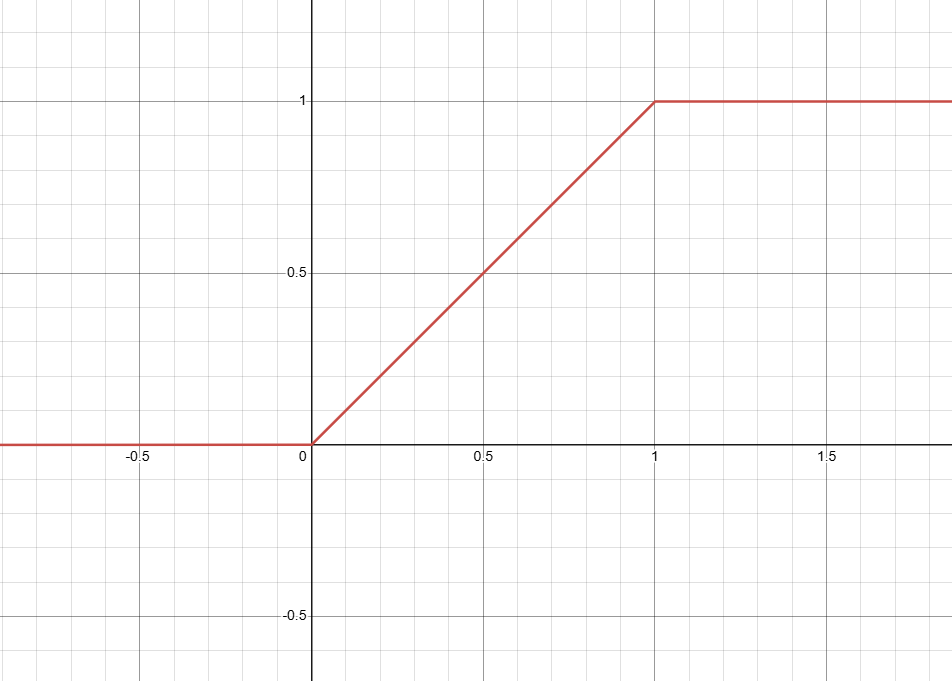
\includegraphics[width=0.9\linewidth]{Reinforcement Learning/Curse of Dimensionality/relusig.png}
        \caption{Caption}
        \label{fig:enter-label}
    \end{figure}
\end{frame}

\begin{frame}{Barron 1993 - function class}
Let $\Gamma_c$ be the set of functions $f$ on $\mathbb{R}^d$ for which there exists a complex-valued Fourier transform measure $\hat F(d\omega)$ such that
$$
f(x) = \int_{\mathbb{R}^d} e^{i\omega\cdot x} \hat F(d\omega)
$$
with the first moment of the Fourier magnitude distribution bounded by
$$
C_f = \int_{\mathbb{R}^d} |\omega||\hat F(d\omega)| \le C
$$
where $|\omega|$ represents the Euclidean norm of the frequency vector.
For a bounded set $B\subset\mathbb{R}^d$ containing the origin $\Gamma_{C,B}$ is the set of functions $f$ on $B$ that can be represented by the above integrals for $x\in B$ with
$$
C_{f,B} = \int \sup_{x\in B} |\omega \cdot x| |\hat F(d\omega)|\le C
$$
    
\end{frame}

\begin{frame}{Interpretation of $C_f$ and $C_{f,B}$}
\begin{itemize}
    \item It is an average of the norm of the frequency vector weighted by the Fourier distribution
    $$
C_f = \int_{\mathbb{R}^d} |\omega||\hat F(d\omega)| \le C
$$
\item It measure the extend the function oscillates
\end{itemize}
    
\end{frame}

\begin{frame}{Example that does not work - $\sin(1/x)$}
    \begin{figure}
        \centering
        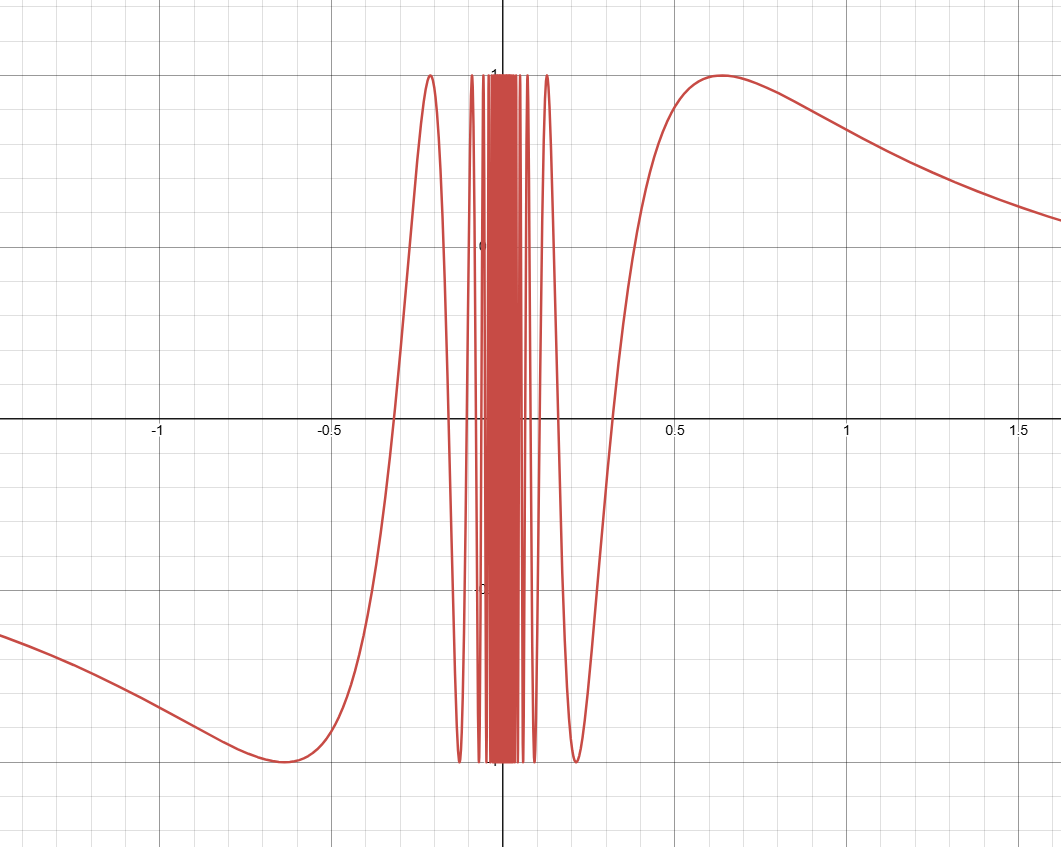
\includegraphics[width=0.6\linewidth]{Reinforcement Learning/Curse of Dimensionality/sin1_x.png}
    \end{figure}
\end{frame}

\begin{frame}{Barron 1993 - Key theorem}
\begin{theorem}
    For every function $f$ with finite $C_f$ and every $n\ge 1$, there exists a neural network with one hidden layer of $n$-sigmoidal nodes:
    $$
    f_n(x) = \sum_{k=1}^n c_k\phi(a_k \cdot x + b_k)+c_0
    $$
    such that the approximation error with respect to any probability measure $\mu$ on the ball $B_r = \{x: |x|\le r\}$ satisfies
    $$
    \int (f(x)-f_n(x))^2 \, \mu(dx) \le \frac{(2rC_f)^2}{n}
    $$
\end{theorem}
\textbf{Remark:} the dimension $d$ doesn't matter with  approximation error of $\mathcal{O}(1/n)$. One caveat: be careful with $C_f$ that depends on $d$.
    
\end{frame}

\begin{frame}{Barron 1993 - function class}
What kind of functions are in this class?
\begin{itemize}
    \item Gaussian function
    $$
    f(x) = e^{-|x|^2/2},\quad C_f\le \sqrt{d}
    $$
    \item Positive definite functions $f(x)$ on $\mathbb{R}^d$
    $$
    \sum_{i,j} \alpha_i\alpha_j f(x_i-x_j)\ge 0
    $$
    for all choices of points and scalars.
    \begin{itemize}
        \item Covariance functions; 
        \item Characteristic functions
    \end{itemize}
    
\end{itemize}

\end{frame}
\begin{frame}{Gaussian}
\begin{figure}
    \centering
    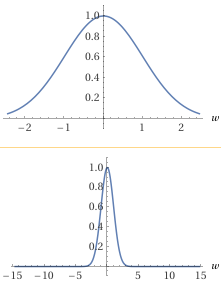
\includegraphics[width=0.3\linewidth]{Reinforcement Learning/Curse of Dimensionality/gaussian.png}
\end{figure}
    
\end{frame}
\begin{frame}{Barron 1993 - function class}
\begin{itemize}
    \item Ridge functions
    $$
    f(x) = g(a\cdot x),\quad a\in\mathbb{R}^d, |a|=1, \quad g\text{ univariate}
    $$
    \textbf{Remark}: This type is particular good as $C_f$ is independent $d$.
    \item \textcolor{blue}{Sigmoidal network with smooth activation function} (has limitation as discussed below)
    \item Radial function
    $$
    f(x) = g(|x|)
    $$
    \item Linear functions, quadratic forms, polynomials, step functions
\end{itemize}
\end{frame}
\begin{frame}{Barron 1993 - functions}
\begin{itemize}
    \item Sufficiently smooth functions: $C^{\lfloor d/2\rfloor+2}$ ($\mathbb{R}^d$)
    \item Boolean functions: functions defined on domain $\{0,1\}^d$
\end{itemize}
    
\end{frame}


\begin{frame}{Barron 1993 - Key message}
\begin{itemize}
    \item For Barron class functions, single hidden layer net achieve approximation error of order $\mathcal{O}(1/n)$ for any dimension $d$
    \item Using fixed basis functions (polynomial, etc), the error cannot be smaller than $\mathcal{O}(1/n^{2/d})$
\end{itemize}
    \textbf{Remark}: $d=1000$, for $\epsilon = 10^{-5}$, need 
\begin{itemize}
    \item NN: $N = 10^5$ nodes for any dimensions
    \item Fixed basis we need $N_{fb} = 10^{5\times 1000/2} =10^{2500}$ basis functions
\end{itemize}
\end{frame}

\begin{frame}{Poggio et al 2017}
Main message: Deep convolutional net have the theoretical guarantee which shallow nets do not have: they can avoid the curse of dimensionality for compositional functions.
\begin{itemize}
    \item The most interesting set of problems consists of compositional functions composed of a hierarchy of constituent functions that are local: An example is 
    $$
    f(x_1,\cdots, x_8) = h_3(h_{21}(x_1,x_2), h_{12}(x_3,x_4), h_{22}(h_{13}(x_5,x_6), h_{14}(x_7,x_8)))
    $$
    \item Key aspect of convolutional network that can given them an exponential advantage is not weight sharing but locality at each level of the hierarchy.
\end{itemize}
    
\end{frame}

\begin{frame}{Poggio et al 2017 - Compositional functions with Binary tree structure}
The function is composed of with functions in a binary tree structure (each take 2 inputs and 1 outputs)
    $$
    f(x_1,\cdots, x_8) = h_3(h_{21}(x_1,x_2), h_{12}(x_3,x_4), h_{22}(h_{13}(x_5,x_6), h_{14}(x_7,x_8)))
    $$
\begin{center}
    \begin{forest}
  [$h_3$
    [$h_{21}$
      [$h_{11}$
        [$x_1$]
        [$x_2$]
      ]
      [$h_{12}$
        [$x_3$]
        [$x_4$]
      ]
    ]
    [$h_{22}$
      [$h_{13}$
        [$x_5$]
        [$x_6$]
      ]
      [$h_{14}$
        [$x_7$]
        [$x_8$]
      ]
    ]
  ]
\end{forest}
\end{center}

\end{frame}

\begin{frame}{Poggio et al 2017 - General compositional function}
For general function with directed acyclic graph, i.e., 
    \begin{center}
        \begin{forest}
  [$h_3$
    [$h_{21}$
      [$h_{11}$
        [$x_1$]
        [$x_2$]
      ]
      [$h_{12}$
        [$x_3$]
        [$x_4$]
      ]
    ]
    [$h_{22}$
      [$h_{13}$
        [$x_5$]
        [$x_6$]
      ]
    ]
  ]
\end{forest}

    \end{center}
\end{frame}
\begin{frame}{Poggio et al 2017 - function class}
Since $f$ is unknown, we need to make some assumptions on the class of functions from whih the unknown target function is chosen. 
\begin{itemize}
    \item $f\in W^{d}_m$: functions of $n$ variables with continuous partial derivatives of order up to $m$
    \item $f\in W^{d,2}_{m}$: compositional functions with binary tree architecture where consituent functions are in $W^2_m$
    \item Argument: many real-world functions have this compositional structure where each constituent function depends on only a small number of variables
\end{itemize}
\end{frame}
\begin{frame}{Poggio et al 2017 - complexity}
    Let 
    \begin{itemize}
        \item $N$: total number of nodes in a network
        \item $V_N$: set of all networks given with total number of nodes $N$
        \item $V_N\subset V_{N+1}$
        \item The degree of approximation is defined by 
        $$
        dist(f,V_n) = \inf_{P\in V_N} \|f-P\|
        $$
        \item For example if $dist(f, V_n) = \mathcal{O}(N^{-\gamma})$ for some $\gamma>0$, then a network with nodes $N = \mathcal{O}(\epsilon^{-1/\gamma})$ will be sufficient to gurantee an approximation with accuracy at least $\epsilon$
    \end{itemize}
\end{frame}
\begin{frame}{Poggio et al 2017 - Key theoerm 1}
\begin{theorem}[Shallow network leads to CoD]
    For general functions $f\in W_m^d$, shallow networks requires
    $$
    N = \mathcal{O}(\epsilon ^{-d/m})
    $$
    nodes to achieve accuracy $\epsilon$. This implies CoD.
\end{theorem}
    \textbf{Remark}: Let $\epsilon = 10^{-5}$, i.e., for a $d$-dimensional $C^m$ function, use shallow network to approximate with error $10^{-5}$ need nodes of order 
    $$
    (10^{-5})^{-d/m} = 10^{5d/m}
    $$
    \begin{itemize}
        \item For $d=10, m=1$, $(10^{-5})^{-10} = 10^{50}$
        \item For $d=100, m=1$, $(10^{-5})^{-100} = 10^{500}$
    \end{itemize}
\end{frame}
\begin{frame}{Poggio et al 2017 - key theorem 2}
\begin{theorem}[Deep network with Binary Tree structure]
For compositional functions $f\in W^{d,2}_m$, deep networks need only
$$
N = \mathcal{O}((d-1)\epsilon^{-2/m})
$$
nodes to achieve approximation error $\epsilon$. 
\end{theorem}
\textbf{Remark}: Note here we have linear dependency on input. Let $\epsilon = 10^{-5}$, i.e., for a $d$-dimensional $C^m$ function with binary tree structure, we need 
$$
(d-1)\times (10^{-5})^{-2/m}) = (d-1)\times 10^{10/m}
$$
\begin{itemize}
    \item For $d=10, m=1$, $(10-1)\times (10^{-5})^{-2/m} = 9\times 10^{10}$
    \item For $d=100, m=1$, $(100-1)\times (10^{-5})^{-2/m} = 99\times 10^{10}$
\end{itemize}
\end{frame}
\begin{frame}{Poggio et al 2017 - key theorem 3}
    \begin{theorem}[General compositional functions]
    For functions with general directed acyclic graph structure, deep network requires
    $$
    N = \mathcal{O}(\sum_{v} \epsilon^{-d_v/m_v})
    $$
    where $d_v, m_v$ is the number of inputs and smoothness parameter to each constituent functions
    \end{theorem}
    \textbf{Remark}: If we have same smoothness level, then
    $$
    N = \mathcal{O}(\sum_{v} \epsilon^{-d_v/m_v}) = \mathcal{O}(\epsilon^{-\max_v dv/mv})
    $$
\end{frame}
\begin{frame}{Poggio et al 2017 - Key message}
\begin{itemize}
    \item For compositional functions, local dimensionality matters
    \item If the function is very smooth, CoD is less severe.
\end{itemize}
    
\end{frame}
% \begin{frame}{Bach 2017 - Setup}
% \begin{itemize}
%     \item Single hiddne layer neural networks
%     \item A hidden layer with $k$ nodes
%     \item Each node computes
%     $$
%     \sigma(w_j^Tx+b_j)
%     $$
%     where $w_j$: weight vector of node $j$, $b_j$: bias of node $j$. 
%     \item $\sigma$ is the activation function, focus on ReLu $\max\{0,x\}$
%     \item The neurel network output is
%     $$
%     f(x) = \sum_{j=1}^k\eta_j \sigma(w_j^Tx+b_j)
%     $$
% \end{itemize}
    
% \end{frame}
% \begin{frame}{Bach 2017 - Key message}
% \begin{itemize}
%     \item If the function adaptive to unknown underlying linear structures such as the dependence on the projection of the input ariables onto a low-dimensional subspace. 
% \end{itemize}
    
% \end{frame}

% \begin{frame}{Bach 2017 - Setup}
% For finite number of nodes, we train by adjusting $w_j, b_j, \eta_j$.
% \begin{itemize}
%     \item Bach 2017 consider we have a continuous set $V$ of possible nodes
%     \item Each node is identified by its parameter $v=(w,b)\in V$.
%     \item Use a measure $\mu$ to tell how much each node contribute
%     \item network output: 
%     $$
%     f(x) = \int_V \sigma(w^T x+b)\,d\mu(w,b)
%     $$
%     \item $\mu$ is like a weight function over all possible neurons
% \end{itemize}
    
% \end{frame}
% \begin{frame}{Bach 2017 - variational norm}
% \begin{itemize}
%     \item Let $V$ be a compact topological space and 
%     $$
%     \{\varphi_v: X\to\mathbb{R}\}_{v\in V}
%     $$
%     be a family of nodes parameterized by $v\in V$.
%     \item The function space $F_1$ is defined as the set of all functions $f:X\to\mathbb{R}$ that can be represented as
%     $$
%     f(x) = \int_V \phi_v(x)\, d\mu(v)
%     $$
%     where $\mu$ is a signed Radon measure on $V$ with finite total variation $|\mu|(V)$.
% \end{itemize}
    
% \end{frame}
% \begin{frame}{Bach 2017 - Variational norm}
% The variational norm $\gamma_1(f)$ is formally defined as
% $$
% \gamma_1(f) = \inf\{|\mu|(V): f(x)= \int_V\phi_v(x)\, d\mu(v)\,\text{for all $x\in X$}\}
% $$
% that is the infimum of the total variation $|\mu|(V)$ over all possible signed Radon measure $\mu$ that represent the function $f$.
    
% \end{frame}

% \begin{frame}{Bach 2017 - Total variation of a measure}
% The total variation $|\mu|(V)$ of a signed Radon measure $\mu$ is defined as
% $$
% |\mu|(V) = \sup\left\{\int_V g(v)\, d\mu(v): g\text{ is continuous with $|g(v)|\le 1$ for all $v\in V$}\right\}
% $$
% Heuristically, this measures the size of $\mu$ by testing it againt all bounded continuous functions.
% \end{frame}
% \begin{frame}{Special case: Density representation}
% When the measure $\mu$ has a density $p$ with respect to a probability measure $\tau$, i.e., $d\mu(v) = p(v)\, d\tau(v)$, then the variation norm simplifies to
% $$
% \gamma_1(f) = \inf\left\{\int_V|p(v)|\, d\tau(v): f(x) = \int_V \phi_v(x)p(x)\, d\tau(v)\text{ for all $x\in X$}\right\}
% $$
% which is the $L^1$ norm of of the density function $p$
 
% \end{frame}
% \begin{frame}{Bach 2017 - Finite Neuron case}
% For the specific case where $f$ is represented by finitely many neurons,
% $$
% f(x) = \sum_{j=1}^k \eta_j\varphi_{v,j}(x)
% $$
% this correspond to 
% $$
% \mu = \sum_{j=1}^k \eta_j \mathbf{1}(v=v_j)
% $$
% and total variation is
% $$
% |\mu|(V) = \sum_{j=1}^k|\eta_j|
% $$
    
% \end{frame}
% \begin{frame}{Bach 2017 - Function class}
% The function class considered in Bach 2017 is denoted as $F_1$, all the functions that can be represented as
% $$
% f(x) =\int_V \sigma(w^\top x+ b)\, d\mu(w,b)
% $$
% i.e., all the functions that can be expressed as possibly infinitely weighted combinations of neurons.
% \begin{itemize}
%     \item Each function $f\in F_1$ has a complexity measure $\gamma_1(f)$
%     \item The smaller $\gamma_1(f)$ is, the simpler the function. 
% \end{itemize}
    
% \end{frame}

\begin{frame}{Are these applicable to macro?}
    \begin{itemize}
        \item Is the policy function smooth?
        \item Does the policy function has finite mean in Fourier distribution
        \item Does the policy function have low local dimensions?
    \end{itemize}
\end{frame}

\end{document}
